% This is file JFM2esam.tex
% first release v1.0, 20th October 1996
%       release v1.01, 29th October 1996
%       release v1.1, 25th June 1997
%       release v2.0, 27th July 2004
%       release v3.0, 16th July 2014
%   (based on JFMsampl.tex v1.3 for LaTeX2.09)
% Copyright (C) 1996, 1997, 2014 Cambridge University Press

\documentclass{jfm}
\usepackage{graphicx}
\usepackage{epstopdf, epsfig, subfigure}

% Macros for consistent formatting
\newcommand*{\fig}[1]{Fig.~\ref{#1}}
\newcommand*{\sect}[1]{\S\ref{#1}}
\newcommand*{\eq}[1]{Eqn.~\ref{#1}}

\title{Aeroacoustic Source Mechanisms in High-Speed Jets}

\author{Michael Crawley\aff{1},
  Lior Gefen\aff{2},
  Ching-Wen Kuo\aff{3},
  Mo Samimy\aff{3}\corresp{\email{Samimy.1@osu.edu}}
 \and Roberto Camussi\aff{2}}

\affiliation{\aff{1}Air Force Research Laboratory, Munitions Directorate, Eglin AFB 32542, USA
\aff{2}Universit\`{a} degli studi Roma Tre, Dipartimento di Ingegneria, Via della Vasca Navale, 79, 00146 Roma, Italia.
\aff{3}Department of Mechanical and Aerospace Engineering, The Ohio State University, Columbus, OH, USA}

\begin{document}

\maketitle

\begin{abstract}
This work aims to study the dynamics of, and noise generated by, the large-scale structures in high-fidelity in a Mach 0.9 turbulent jet using plasma-based excitation to produce either individual or periodic coherent ring vortices in the shear layer.
First, two-point cross-correlations are used between the acoustic near-field and far-field in order to identify the dominant noise source region.
The large-scale structure interactions are then investigated by stochastically-estimating the time-resolved velocity fields from time-resolved near-field pressure traces and non-time-resolved planar velocity snapshots using an artificial neural network.
Finally, from the estimated time-resolved velocity the aeroacoustic source terms were computed using Ribner's dilatation-based acoustic analogy.
The results indicated that the disintegration of the coherent ring vortices are the dominant aeroacoustic source mechanism for the jet studied here. 
However, the merging of vortices in the initial shear layer was also identified as a non-trivial noise source mechanism. 
\end{abstract}

\begin{keywords}

\end{keywords}

\section{Introduction}
\label{introduction}
The advent of the turbojet engine led to a transformation in both commercial and military aviation, allowing for much faster flight than previously possible with propeller-driven aircraft. 
However, the increased thrust of turbojets has come at great cost; significant acoustic radiation is generated by the rotating components (compressor, turbine, fan), by the combustion process, and ultimately by the free jet itself. 
This has spurred extensive research into the acoustic source mechanism in high speed, high Reynolds number jets, and while progress has been made in the field of aeroacoustics, understanding of jet noise sources and their radiation mechanisms remains incomplete \citep{Jordan2008}.
This is due to the large number of interrelated parameters (e.g. Reynolds number, temperature ratio, acoustic Mach number, nozzle geometry, et cetera) as well as the large disparity in the associated length and time scales of the turbulent phenomena and the radiated noise.
As a result, current noise-mitigation technologies for free jets have largely been applied in an ad
hoc manner, due to the community's incomplete understanding of the aeroacoustic sources.
Fully realizing this maximum noise reduction potential will require a much more detailed understanding of the mechanism (or mechanisms) by which free jets radiate to the far-field.

It is generally agreed that the dominant noise sources in high-speed jets are related to the large-scale coherent structures which have been identified in the jet mixing layer \citep{Arndt1997}. 
As discussed by \citet{Tam1995} (among many others), large-scale structures can be represented as instability waves superimposed upon the mean flow.
At subsonic convection velocities, a plane instability wave with fixed frequency-wavenumber will emit no acoustic radiation to the far-field.
However, modulation of the instability wave's amplitude creates a dispersion in the energy content of the instability wave.
By doing so, the broadband instability wave, commonly referred to as a \emph{wavepacket}, can shift energy to supersonic phase-velocities and hence produce sound which radiates to the far-field.
Wavepacket models for noise emission have become commonplace, owing to their great success at predicting low-angle acoustic emission \citep{Obrist2011}.
Simple linear wavepacket models have allowed researchers to probe different aspects of the waveform modulation, in turn illuminating possible relevant dynamical behavior of the large-scale structures for the noise generation process.
Temporal modulation of the wavepacket's amplitude and spatial extent (`jittering') were shown to increase the efficiency of the noise source \citep{Cavalieri2010}; this conforms to experimental results which have indicated that the noise generation in free jets is highly intermittent \citep{Hileman2005,Kearney-Fischer2013}. 
Though progress has been made in experimentally measuring wavepacket characteristics in high-speed turbulent jets \citep{Cavalieri2013,Baqui2014}, a direct link between large-scale structure dynamics and the aeroacoustic source has remained elusive.

In tandem to instability analysis of the noise source mechanism, the development and refinement of acoustic analogies has occurred. 
\citet{Lighthill1952} was the first to reorganize the Navier-Stokes equations into a linear wave equation with a quadrupole-like source term comprising density, Reynolds stress, and entropic fluctuations.
Work by \citet{Phillips1960}, \citet{Lilley1974}, and much later \citet{Goldstein2003} extended this formulation to include convective effects of the ambient medium, thereby separating the true sound sources in Lighthill's acoustic analogy from purely propagative effects.
Competing variations were also developed by \citet{Powell1964}, \citet{Howe1975}, and \citet{Ribner1962} (the last of which will be used in the current work) which sought to better connect the acoustic source mechanisms to distinct physical phenomena occurring in the turbulent shear layer.
In a similar vein, \citet{Cabana2008} decomposed Lighthill's acoustic source term into sub-terms of velocity, vorticity, dilatation and density fields in order to understand the relative (and sometimes competing) roles each had the the noise generation process.
Ultimately however, a clear distinction between efficiently and non-efficiently radiating structures has not been defined.

The purpose of this work is to examine the dynamical evolutions of the large-scale coherent structures which lead to the dominant mixing noise in the subsonic, turbulent jet.
The focus will be on the axisymmetric, toroidal vortices (azimuthal Fourier mode zero), as these are known to dominant the acoustic far-field.
The jet will therefore be excited using localized arc-filament plasma actuators in order to generate these axisymmetric structures with a well-defined temporal frequency and phase.
The irrotational near-field pressure will be acquired via a linear array of microphones, and decomposed into its constitutive acoustic and hydrodynamic components in order to identify the dominant noise source region.
Time-resolved velocity fields will then be estimated based on stochastic correlations between the near-field pressure and the orthogonal modes of ensemble (non-time-resolved) velocity field, identified by an artificial neural network.
From these time resolved fields, the coherent structure dynamics will be identified.
Lastly, the aeroacoustic source field will be computed using Ribner's Dilatation acoustic analogy \citep{Ribner1962}.
In doing so, the structure dynamics will be directly linked first to the acoustic source region, and finally to the acoustic sources themselves.
\include{sect_methodology}
\section{The Near- and Far-field Response to Excitation}
\label{sect:nearfield}
\subsection{Periodic and Impulse Response}
The genesis for this project first began with the work of \citet{Sinha2012}, which studied the irrotational near-field response of a subsonic jet subjected to excitation with plasma actuators by decomposing the instantaneous fluctuating pressure field into a coherent `wave' component (which corresponds to the large-scale structure generated by the excitation) and incoherent residual fluctuations (which correspond to the natural turbulence in the jet). 
Fundamentally, this decomposition is similar to the triple decomposition used by \citet{Hussain1970}.
Sinha \etal found that each pulse from the actuators produces a coherent large-scale structure that would grow, saturate, and decay as it advects through the jet shear layer. 

In the irrotational near-field, the signature of these large-scale structures takes the form of a compact waveform. 
At low enough excitation frequencies, the characteristic period of this waveform is much less than the excitation period, and hence, the structures seeded by the excitation do not interact with one another as they evolve downstream. 
Therefore, their behavior can be thought of as representing the response of the jet to a single perturbation; in short this is the `impulse' response of the jet, which is produced by the impulsive excitation by LAFPAs.
As the period of actuation approaches the characteristic period of the impulse response, the waveforms extracted by the phase-averaging technique are largely unmodified from that of the impulse response. 
Above this frequency, significant interaction between the structures is observed, with noticeable modifications to the waveform shape and amplitude. 
As the structures are growing as they advect through the shear layer, the frequency at which the structures begin to interact is dependent on the axial location.
This behavior can be observed in \fig{fig:ch3_nearfield}a.
\begin{figure}
	\centering
%	\begin{subfigure}{.5\textwidth}
%		\centering
		\includegraphics[width=0.45\linewidth]{Figures/ch3_nearfield_phavg_v2.png}
%		\caption{}
%		\label{fig:ch3_nearfield_phavg}
%	\end{subfigure}%
%	\begin{subfigure}{.5\textwidth}
%		\centering
		\includegraphics[width=0.45\linewidth]{Figures/ch3_nearfield_linear_v2.png}
%		\caption{}
%		\label{fig:ch3_nearfield_linear}
%	\end{subfigure}
	\caption{Phase-averaged waveforms along the first array position at $x/D = 3, r/D = 1.35$ (a) and a linear superposition of the phase-averaged waveform for the impulse excitation ($St_{DF} = 0.05$) compared against periodic excitation ($St_{DF} = 0.50$) (b).}
	\label{fig:ch3_nearfield}
\end{figure}

For a certain range of excitation frequencies ($St_{DF} \leq 0.50$ at $x/D = 2$, for example), the structures interact in a quasi-linear manner, insofar as their near-field pressure signatures are concerned. 
To be precise, the response of the jet in the irrotational near-field could be well-predicted by a linear summation of the impulse response of the jet, repeated at the periodic excitation frequency. 
This concept has been illustrated in \fig{fig:ch3_nearfield}b, where the periodic response of the jet to excitation with $St_{DF} = 0.50$ has been reproduced at $x/D = 3$. 
Additionally, a linear superposition of the impulse response for $St_{DF} = 0.05$, repeated to match the excitation frequency of $St_{DF} = 0.50$, has been overlaid. 
The linear superposition has been arbitrarily shifted in time in order to match the phase of the periodic response; this phase difference is likely due to the dependence of convection velocities on structure frequency \citep{Veltin2011} (or more accurately, structure size). 
For reference, the impulse response has also been included in the plots. 
Upstream of the end of the potential core ($x/D \simeq 6$, as will be found in \sect{sect:velocity}), the quasi-linear interaction model produces close predictions of the waveform amplitude and shape, despite the significant difference in both peak amplitude and waveform shape between the impulse and periodic responses. 

This quasi-linear interaction of the jet response to excitation is not limited exclusively to the hydrodynamically-dominated regions of the jet, but in fact holds for the acoustic far-field as well, at aft angles (where the acoustic signal is strongest and is known to correlate well with large-scale structures). 
This can be observed in \fig{fig:ch3_farfield}a, where the phase-averaged response of the jet has been plotted for the far-field signal at a polar angle of $30^\circ$. 
For legibility, only a select number of excitation Strouhal numbers have been included. 
As with the irrotational near field, the acoustic far field exhibits a compact waveform for the lowest excitation Strouhal numbers. 
Though nearly a direct inverse from the waveform observed in the hydrodynamically-dominated near field, the far-field waveform is quite reminiscent of the phase-averaged waveforms observed by \citet{Kambe1983} for the acoustic radiation towards aft angles produced by the head-on collision of vortex rings. 
At higher $St_{DF}$, a continuous oscillation between sharp expansion and compression waves is again observed, though the amplitude begins to decay above moderate excitation Strouhal numbers. 
\begin{figure}
	\centering
%	\begin{subfigure}{.5\textwidth}
%		\centering
		\includegraphics[width=0.45\linewidth]{Figures/ch3_farfield_phavg_v2.png}
%		\caption{}
%		\label{fig:ch3_farfield_phavg}
%	\end{subfigure}%
%	\begin{subfigure}{.5\textwidth}
%		\centering
		\includegraphics[width=0.45\linewidth]{Figures/ch3_farfield_linear_v2.png}
%		\caption{}
%		\label{fig:ch3_farfield_linear}
%	\end{subfigure}
	\caption{Phase-averaged waveforms of the far-field at $30^\circ$ (a) and a linear superposition of the phase-averaged waveform for the impulse excitation ($St_{DF} = 0.05$) compared against periodic excitation ($St_{DF} = 0.25$) (b).}
	\label{fig:ch3_farfield}
\end{figure}

As before, a linear superposition of the impulse response can well predict the waveform shape and amplitude at the higher excitation frequencies (\fig{fig:ch3_farfield}b), though in this case only up to $St_{DF}  = 0.25$. 
From the phase-averaged waveforms alone it is not clear whether this breakdown in the linear superposition model at the highest excitation frequencies is due to nonlinear behavior or uncertainty in the phase-averaging. 
Results comparing the linear superposition of the impulse response against the measured periodic response at $St_{DF}  = 0.35$ are shown in \fig{fig:ch3_farfield_nonlinear}.
Some similarities may be found in the waveform shape and amplitude, but overall it is clear that the acoustic response of the jet to excitation at $St_{DF}  = 0.35$ is substantially modified from the response at lower frequencies.
Though this is hardly conclusive in its own right, this result does suggest either changing or competing acoustic source mechanisms are present in these excited jets.
The phase-averaged waveforms were also investigated at polar angles of $60^\circ$ and $90^\circ$; however a clear waveform was not identifiable over the statistical uncertainty inherent in the phase-averaging process (likely due to the superdirective character of the acoustic radiation \citep{Crighton1990}, which renders the amplitude at sideline angles too low to be detectable).
Additional details and analysis of the phase-averaged near- and far-field signals can be found in \citet{Crawley2015}.
\begin{figure}
	\centering
	\includegraphics[width=0.45\linewidth]{Figures/ch3_farfield_linearsuperposition_st035_v2.png}
	\caption{Linear superposition of the phase-averaged impulse response to excitation against the measured periodic response for $St_{DF} = 0.35$ at the  $30^\circ$ far-field microphone.}
	\label{fig:ch3_farfield_nonlinear}
\end{figure}

\subsection{Excited versus Natural Structures}
As the forced large scale turbulent structures propogate downstream, they produce a nearfield pressure wave signature that has been shown in figure \ref{fig:phaseaxialbothM} for three different excitations, $St_D \in \{ 0.05, 0.15, 0.25 \}$ in the phase-averaged sense. 

It is not possible to use phase--averaging with the unforced case since the structures, although dominated by Strouhal numbers related to the instabilities in the jet, experience enough variation that they can not be captured using phase-averaging at a specific frequency. 
It is necessary to use an alternative averaging method in order to appreciate a similar signature due to unforced jet turbulent--structures.
Instead of phase-averaging, a wavelet--based method, namely wavelet--conditioning, was applied to the unforced and forced cases to determine how closely the forced structures relate to the natural structures in the jet for both the experiments and simulations.

\subsubsection{Wavelet Conditioning Process}
The wavelet--conditioning was used for structure identification in jets and other turbulent flows \citep{Camussi1997,Camussi1997b,Guj1999,Camussi2002,Guj2003}.
The technique is based on the use of the so--called Local Intermittency Measure or LIM, introduced in 1992 by \citet{Farge1992}.
The LIM is the ratio between two energies: a local energy for a specific time and scale $(\tau, s)$ and an averaged energy in time for the same scale $s$.
The LIM was demonstrated to be a well suited indicator for coherent structure identification \citet{Camussi1997}. Its mathematical expression is:
\begin{equation}
\label{eqn:LIM}
L(s, \tau) = \frac{w^{2}(s, \tau)}{\left<w^{2}(s, \tau)\right>_{\tau}}
\end{equation}
where $w^{2}(s, \tau)$ is the local energy for a specific time and scale, and $\left< \bullet \right>_{\tau}$ represents a time average.
As a ratio between positive quantities, LIM can only be positive ($L \geqslant 0 $). LIM gives an information about the fluctuation of energy and by choosing a proper threshold $T$ it is possible to select a set of times $\{\tau_{i}\}$ corresponding to peaks with value greater than the threshold $T$.
The peaks are local maxima of LIM and are constrained by the following conditions:
\begin{equation}
		\begin{array}{ll}
			& L(s, \tau) > T,\\
			\\
			& \frac{\partial L}{\partial \tau}(s, \tau) = 0,\\
			\\
			&\frac{\partial^{2} L}{\partial \tau^{2}}(s, \tau) < 0.
		\end{array}
\end{equation}

An iterative process was used in order to fix the threshold, $T$. To initiate the iterative process it is needed first to select a 'first estimate' of the threshold. It was taken to be equal to 1. The algorithm of the iterative process is applied to each scale of the wavelet--decomposition and allows to have a threshold for each scale. The algorithm used to obtain this is:
\begin{enumerate}
	\item Select a first threshold to initiate the iterative process (1 in the present case)
	\item Evaluate the coefficient
	\begin{equation}
	R(T) = -\frac{\log\left(\frac{N_p}{N_m}\right)}{\log\left(\frac{\sigma_{w_p}}{\sigma_{w_m}}\right)}
	\end{equation}
	\item Re-evaluate $T$
	\item Iterate points 2 and 3 until $T$ achieve the maximum of $L$ for the scale under analysis
\end{enumerate}
where $N_p$ is the length of the set $\{L > T\}$, $N_m$ is the length of the set $\{L \leqslant T\}$, $\sigma_{w_p}$ the standard deviation of the set $\{w\left( \tau_p\right) | L\left( \tau_p \right) > T\}$ and $\sigma_{w_m}$ the standard deviation of the set $\{w\left( \tau_m\right) | L\left( \tau_m \right) \leqslant T\}$.
The outcome of this iterative process is a set of vectors: one containing the different value of $T$ and the second the different value of $R(T)$. The threshold for the analysis is selected to correspond to the maximum of $R(T)$.

The next step is to get similar results to those obtained with the phase--average. In order to get the signatures, a conditional--average (eqn. \ref{eqn:ensembleAverage}) using the set of times $\{\tau_{i}\}$ is performed. In one way, the conditional--average and phase--average are similar: the set of times $\{\tau_{i}\}$ replaces the phases on which the phase--average is performed. At each time location corresponding to a peak of energy, a window $W$ of fixed time--length $l_{W}$ is selected from the original signal $p \left( t \right)$. The conditional--average, $\tilde{p}$ is calculated from this set of windows:
\begin{equation} \label{eqn:ensembleAverage}
	\tilde{p}^n_{m}\left( W \right) = \left< p_{m} | P_{k} \right>_{\tilde{\tau}^n_{s}} = \frac{1}{N^n} \sum^{N^n}_{i = 1} p_{m}\left(\xi_{i}\right),
\end{equation}
where the superscript $n$ and subscript $m$ stand for the position of the reference signal and of any other signal of the array, respectively. Also, the subscript $s$ stands for the scale, $N^n$ is the number of detected events, $\tilde{\tau}^n_{s}$ is the set of corresponding times for a specific scale $s$ at which these events are occurring and $\{\xi_{i}\}$ is the interval surrounding each peak, $\xi_{i} \in \left[ \tilde{t}_{i} - \frac{l_W}{2}, \tilde{t}_{i} + \frac{l_w}{2} \right]$, $\tilde{t}_{i} \in \tilde{\tau}^n_{s}$.
A first analysis using equation \ref{eqn:ensembleAverage} was performed on the microphones line--array. A second analysis was then performed by doing the conditional--average only with peaks with negative/positive value in the real domain (pressure).

%\begin{figure}
%	\centering{}
%	\subfloat[only negative peaks]{\includegraphics[width=3.2in]{figures/eps/negativePeak.eps}}
%	\subfloat[only positive peaks]{\includegraphics[width=3.2in]{figures/eps/positivePeak.eps}}
%	
%	\subfloat[comparison between the signatures]{\includegraphics[width=3.2in]{figures/eps/compPeaks}}
%	\caption{Auto--conditioning signatures of the signal at $x/D = 3$} \label{fig:compPeaks}
%\end{figure}
%Figure \ref{fig:compPeaks} presents the two subfigures for the different cases (negative/positive peaks) and a third subfigure to compare them.
%%\begin{itemize}
%%  \item $(a)$ conditional--average (eqn. \ref{eqn:ensembleAverage}) using only the negative peaks
%%  \item $(b)$ only the positive peaks
%%  \item a comparison between the two previous one ($(a)$ was inverted in order to compare it to $(b)$)
%%\end{itemize}
%Figure \ref{fig:compPeaks}$(c)$ presents the resemblance between the signature of subfigures $(a)$ and $(b)$ on which the conditional--average was performed using only negative or positive peaks (it is important to understand that the differentiation is done by evaluating the value of each peak in the real domain and not in the LIM/wavelet domain). At this point, it is believed to be the result of the passage of two sucessive large scale turbulent--structures, in the zone where their interaction take place.
%% Do you think I should put a scheme here to explain it?
%The formulation of the conditional--average was modified to take this observation into account and reformulated as follows:
%\begin{equation} \label{eqn:condAvgSign}
%\tilde{p}_{m}^n\left( W \right) = \left< p_{m} | P_{k} \right>_{\tilde{\tau}^n_{s}} = \frac{1}{N^n} \sum^{N^n}_{i = 1} sign\left( p_{n} \left( \tilde{t}_{i} \right) \right) p_{m} \left( \xi_{i} \right),
%\end{equation}
%$sign\left( p_{n} \left( \tilde{t}_{i} \right) \right)$ is introduced to take into account the sign of the peak in the real domain. This operation might be unnecessary for an experimental database (with a long time--series) but for a numerical database which is strongly limited in its time duration it improves the results obtained with the wavelet--conditioning.
%The conditional--average using eqn. \ref{eqn:ensembleAverage} with all the peaks present (not presented here) is not relevant as additional proof for the separation between negative/positive peaks.
%When the conditional--average is performed on a signal $p_{n}$ by using its own set of times ${\tilde{\tau}^n_{s}}$, making $n = m$; it becomes the auto--conditioning. If the conditional--average of a signal $p_{m}$ is done by using the set of times of a signal $p_{n}$, and so $n \neq m$; it is then called the cross--conditioning. The auto/cross--conditioning are presented in Fig.  \ref{fig:condNcond}: the top is the auto--conditioning where the selection of $W$ is done in the reference signal $n$; and the bottom is the cross--conditioning of another signal $m$ where $W$ is centered around the times obtained with signal $n$. For more information about the wavelet--transform, see \cite{Farge1992}.
%\begin{figure}[!ht]
%	\centering
%	\includegraphics[width=1\textwidth]{figures/pdf/condNcond}
%	\caption{\textit{Auto--conditioning of a signal $p_n(t)$ and cross--conditioning of a signal $p_n(t)$}}
%	\label{fig:condNcond}
%\end{figure}

\subsection{Identifying the Acoustic Source Region}
\label{sect:near_field_source_region}
Much of the difficulty in identifying the aeroacoustic source terms revolves around the dissimilar range of scales and fluctuation intensities of the turbulent eddies in the shear layer and the resulting radiated noise. 
Outside the jet shear layer, in the irrotational near-field of the jet, strong hydrodynamic pressure fluctuations associated directly with the passage of coherent structures in the shear layer and their resultant weak acoustic radiation coexist \citep{Arndt1997}. 
Beyond this, in the acoustic far-field, the hydrodynamic signature of the coherent structures is nonexistent owing to their strong exponential decay with radial distance.
Owing to this, identification of pure acoustic waves and their corresponding source events is problematic.
A decomposition of the pressure field into its constitutive hydrodynamic and acoustic components is therefore required. 
By identification and prediction of coherence nulls in the near field, \citet{Coiffet2006} showed that the full irrotational near-field consistent primarily as a linear superposition of its hydrodynamic and acoustic components, which lead subsequent researchers to propose linear filters to extract the individual components from the near-field pressure, with varying degrees of success. 

As discussed by \citet{Tinney2008}, in a transonic jet in which the large-scale structures are convecting subsonically with respect to the ambient speed of sound, a demarcation of the hydrodynamic and acoustic energy fields can be observed with phase velocity.
This is because the hydrodynamic pressure fluctuations will be aligned with the jet axis, and traveling subsonically. 
Acoustic pressure fluctuations will impinge on the linear microphone array at oblique angles, and therefore will appear as having either sonic or supersonic phase velocity, based on the source location. 
Therefore, a demarcaction between the hydrodynamic and acoustic energy components should be readily identifiable about the sonic wavenumber, $k_a = \omega / a_\infty$.
Decomposition of the irrotational near-field pressure is therefore straightforward in Fourier space.

However, there is also a great drawback associated with Fourier analysis: while it analyzes a given signal at a distinct frequency, local information for a given event is spread over all spectral coefficients. 
This is due to the fact that the basis functions used by the Fourier transform oscillate indefinitely. 
For a signal composed of completely random fluctuations this is not an issue, however it has become increasingly clear that the jet noise phenomenon is not a random process \citep{Kearney-Fischer2013}.
Transient events, such as intermittency or the spatial and temporal modulation of a wavepacket, have been shown to be important in the noise generation process. 
It was for this reason that a continuous spatio-temporal wavelet filter, based off of the work of \cite{Antoine2004} and \cite{Kikuchi2010}, was instead used in the current work to decompose the acoustic and hydrodynamic near-fields based on phase-velocity.
It has been shown that by using a temporally/spatially localized fluctuation as a basis, the wavelet transform compresses the information in a turbulent field much more efficiently (and accurately) than the Fourier transform \citep{Farge1992}.
A much more detailed explanation of the spatio-temporal wavelet transform, the justification for its use in decomposing the near-field pressure, and validation of the methodology using the current database can be found in \citet{Crawley2016}. 

By decomposing the irrotational near-field pressure, the relationship between the near- and far-field can be more easily elucidated. 
Two-point correlations were computed using both the full near-field and the acoustic near-field component, between each microphone in the near field and the far-field microphone at $30^\circ$; results can be found in \ref{fig:ch3_full_vs_partial_xcorr}. 
Examination in the spatio-temporal domain shows distinct regions of positive and negative correlation spanning several jet diameters and flow time scales.
The time lag, $\tau$, in the figures have been non-dimensionalized by the ambient speed of sound, $a_\infty$, and $R$, the distance from each near-field microphone to the far-field microphone (note that this results in an ordinate that is scaled separately along the abscissa, due to the dependence of the axial position on $R$).
\begin{figure}
	\centering
		\includegraphics[width=0.475\linewidth]{Figures/sect_nearfield_fullxcorr.png}
		\includegraphics[width=0.401\linewidth]{Figures/sect_nearfield_acousticxcorr.png}
	\caption{Normalized two-point correlations for the natural jet between the near field and the far field at $30^\circ$ for the full near-field pressure (a) and the acoustic component only (b).}
	\label{fig:ch3_full_vs_partial_xcorr}
\end{figure}

Near the jet shear layer (\fig{fig:ch3_full_vs_partial_xcorr}a), four distinct correlation regions can be observed: two positive, two negative; one strong and one weak for each. 
The first correlation regions, the strong-negative and weak-positive, are noticeable beginning at the most upstream microphone and reach their peak values around $5 < x/D < 10$, decaying significantly beyond that.
The slopes of these regions indicate propagation velocities noticeably below the sonic velocity; in the upstream region, they roughly match with the measured convective velocity of the large-scale structures ($U_c \simeq 0.7 U_j$ as measured by two-point correlations between subsequent near-field microphones, see \citet{Crawley2015} for additional details) in the upstream region of the jet, and slowly decelerate downstream.
Similar behavior was observed by \citet{Bogey2007}, who noted that two-point correlations between the flow-field and acoustic near-field in a simulated jet produced strong positive correlation regions which peaked at the end of the potential core and which followed the convection of the large-scale structures.
Conversely, the strong-positive and weak-negative correlation regions exhibit propagation velocities that match well with the ambient speed of sound. 
The distinctly different propagation velocities and of the two pairs of correlation regions indicate that these correspond to different physical phenomena.
The strong-negative and weak-positive correlation regions observed near the jet shear layer are associated with the large-scale structures themselves, rather than acoustic phenomena. 
This relationship becomes even more clear when just the acoustic component of the near-field is considered, rather than the full irrotational near-field. 
Gone entirely now are the correlation regions with subsonic propagation velocities (\fig{fig:ch3_full_vs_partial_xcorr}b), and instead, a single positive correlation region corresponding to sonically-propagating waves exists over the entire domain. 

The correlations of the decomposed near-field can be used to identify the acoustic source region, at least in a rough sense, by comparing the time lag at which the greatest correlation is achieved against expected times-of-arrival for different propagation paths.
A schematic of these propagation paths is provided in \fig{fig:ch3_ToA}.
The first expected time of arrival, $\tau_a$, corresponds to the expected time lag for an acoustic wave traveling directly from the noise source to the near-field microphone and on to the far-field microphone and hence, the noise source region lies along the axis created by the near-field and far-field microphones.
Another expected time-of-arrival can be constructed by assuming the source region is stationary in space; from simple geometric considerations of the distance from the assumed source region to the near-field and far-field microphones, the time lag, $\tau_s$, between the arrival of an acoustic wave at both microphones can be computed.
The stationary source region is of course not known \textit{a priori}, but is set by the author subsequent to the computation of the two-point correlations.

For simplicity, density and convection effects on the acoustic wave as it travels through the jet shear layer have been neglected in this analysis. 
By necessity, it has been assumed that the acoustic radiation in the jet is dominated by $m = 0$ azimuthal Fourier mode (the near-field and far-field microphone arrays are not at the same azimuthal angle with respect to the nozzle). 
This assumption is easily justified in the excited jets, where the actuators have been fired in phase. 
While the near-field pressure and acoustic radiation towards aft polar angles in a natural, high Reynolds number jet is a combination of numerous azimuthal Fourier modes, previous researchers have found these fields to be dominated by the axisymmetric mode \citep{Arndt1997,Hall2006,Koenig2013,Juve1979}.
\begin{figure}
	\centering
	\includegraphics[width=3in]{Figures/ToA_tau.png}
	\caption{Expected times of arrival for on-axis acoustic propagation, $\tau_a$, and off-axis acoustic propagation, $\tau_s$ from a stationary source region centered at $x_s$.}
	\label{fig:ch3_ToA}
\end{figure}

Here, the acoustic source region was assumed to be located at $x_s /D = 4$, which is just upstream of the end of the potential core in the unforced jet. 
(Please note that this analysis is not meant to imply that the source region is located at a specific, fixed point – it is merely a convenient way of understanding the propagation paths.)
Similar behavior is observed between the natural jet and the excited cases in \fig{fig:ch3_xcorrOA}; note that due to numerical discrepancies at the domain boundaries (see \citet{Torrence1998} for a discussion of the `cone of influence' of wavelet coefficients and the effect thereof), the correlation values have been truncated at the most upstream and downstream microphones.
For the impulsively-excited jet, nearly identical correlation regions are observed between the excited and natural jet; in the periodically-excited jet continuous oscillations occur throughout time due to the similarity of continuously-generated large-scale structures and resultant acoustic radiation.
In the upstream region of the jet, the peaks of the positive correlation region match $\tau_a$ nearly exactly. 
In the downstream region, $\tau_a$ begins to increasingly over-predict the time lag for the maximum correlation. 
On the other hand, $\tau_s$ tracks the time lags for the peak correlation consistently over the downstream region, but not the upstream region. 
The results found here appear to indicate that the dominant acoustic radiation reaching the far-field aft angles is being generated over an extended region of the jet mixing layer, roughly $x/D \leq 4$, which is just upstream of the time-averaged end of the potential core in the natural jet.
This is not too dissimilar from the findings of other researchers, who have suggested that the acoustic source region lies just \textit{downstream} of the end of the potential core \citep{Hileman2005}.
It should be clarified here though, that the interpretation of these results is not meant to suggest that only trivial levels of noise are generated outside of this apparent noise source region, just that the dominant radiation is produced in this region in a time-averaged sense.
\begin{figure}
	\centering
	\includegraphics[width=\linewidth]{Figures/sect_nearfield_ffxcorr.png}
	\caption{Normalized two-point correlations between the acoustic component of the near field and the far field at $30^\circ$ for microphone array position starting at $x/D = 1, r/D = 1.2$ for the natural jet (a), $St_{DF} = 0.05$ (b), $St_{DF} = 0.25$ (c) and $St_{DF} = 0.35$ (d).}
	\label{fig:ch3_xcorrOA}
\end{figure}

However, these results should not be interpreted as indicating that the source mechanisms are necessarily consistent for all excitation frequencies. 
For the lower-frequency periodic excitation ($St_{DF} \leq 0.25$), the consistency in the far-field response (\fig{fig:ch3_farfield_linear}) coupled with the consistency in the apparent source region is suggestive of a consistent dominant source mechanism.
In contrast, the inconsistency in the far-field response for the higher-frequency periodic excitation ($St_{DF} \geq 0.35$, \fig{fig:ch3_farfield_nonlinear}) is suggestive of a change in the dominant source mechanism, just one that is associated with the vortex dynamics in the jet shear layer upstream of the end of the potential core.
It should also be noted that the peak correlation values between the acoustic near-field and the far-field are significantly lower (though certainly non-negligible) in the periodic excitation cases, suggesting a decaying coherence in the source mechanisms at these frequencies.
From the current results alone, the significance of this estimated source region is not entirely clear.
In \sect{sect:velocity} the time-resolved velocity field will be explored in detail to better elucidate the structure dynamics, with a particular focus on the region just upstream of the end of the potential core.

The authors would like to make a special note here, concerning the discrepancy between the results presented in \fig{fig:ch3_xcorrOA} and those presented previously in \citet{Crawley2015}.
In that paper, the more simple Fourier filter was used to decompose the irrotational near-field; processing artifacts were noted and a parametric study was attempted to minimize their impact.
In the resulting two-point correlations of the decomposed acoustic field, a shift in the apparent source region was noted to coincide with the shift of the peak pressure fluctuations measured just outside the shear layer (higher frequency excitation cases saturating further upstream near the nozzle exit).
Because this behavior was observed across the entire range of filter parameters used, it was assumed to be representative of the true physical behavior and not a numerical artifact.
Of course, this assumption precludes the possibility that \textit{the entire parameter space produced similar numerical artifacts}. 
As discussed more thoroughly in \citet{Crawley2016}, the Fourier filter has a tendency to allow energy leakage from the hydrodynamic field into the acoustic, particularly at low frequencies. 
Since it has already been observed that the hydrodynamic signature of the large-scale structures can linearly correlate to the acoustic emission, a potential consequence of this leakage is correlation regions which instead point to the region of high hydrodynamic energy - i.e. the saturation point of the near-field pressure fluctuations.
The analysis found of \citet{Crawley2016} demonstrated that wavelet filter is far more robust to energy leakage and numerical artifacts, and as such the authors is inclined to lend more credence to the results presented herein. 
\section{Vortex Dynamics in a Turbulent Mixing Layer}
\label{sect:velocity}
Analysis of the evolution, interaction, and disintegration of the large-scale structures, and ultimately the noise generated thereby, is greatly simplified by the acquisition of time-resolved flow-field measurements.
Furthermore, as will be explained in \sect{sect:source}, computation of the aeroacoustic source field from a simplified acoustic analogy will require time-resolved flow-field data.
Unfortunately, directly acquiring time-resolved velocity fields for the jet currently under study is simply not possible due to the combination of a large domain of interest ($0 \leq x/D \lesssim 12, 0 \leq r/D \lesssim 3$) and high characteristic frequencies on the order of tens of kHz.
Full-field, high-fidelity measurement techniques capable of this required repetition rate were not available to the researchers.
An indirect method is therefore required in order to estimate the evolution of the large-scale structures, in a reduced-order sense.

Phase-locking of a data acquisition system to a reference signal (such as an actuator or a naturally occurring resonance tone) is a common experimental technique, and was initially considered for the present work.
However, sample analysis performed using a numerical database indicated that a very high temporal resolution was required in order to accurately compute fluctuation rates in the dilatation field (the relevance of which will become more apparent in the following section).
At moderate to high excitation frequencies, this was feasible, though potentially tedious (for example, $\sim$16 phases were estimated as necessary at $St_{DF} =0.25$).
At $St_{DF} =0.05$ however, this would require roughly \textit{forty} phases (the significant dead time between actuations means that it is not necessary to acquire the entire range of phases from $0$ to $2\pi$, but this is small consolation).
Clearly, a more efficient data acquisition method is needed.

\subsection{Stochastic Estimation}
The current work borrows heavily from the methodology of \citet{Tinney2008b} and \citet{Sinha2010} in order to estimate the two-component time-resolved velocity field on a streamwise slice of the jet.
The computational methodology by which the stochastic estimation is performed has been modified, however.
Complementary stochastic estimation is used, due to its significantly lower computational cost as well as theorized improvement in accuracy \citep{Bonnet1994}.
The estimated velocity fields produced by LSE were projected onto the POD eigenfunctions (computed from the random, non-time-resolved velocity fields) to produce an estimate of the time-dependent POD coefficients, which can then be used to reconstruct low-order representations of the estimated random velocity field.
Multiple time delays are incorporated, as this has been found to significantly improve the accuracy of the reconstructions for many flow regimes \citep{Ewing1997,Tinney2006,Tinney2008b,Durgesh2010}.
Instead of performing the stochastic estimation using either linear or higher-order cross-correlations (or cross-spectra), the conditional mapping between the near-field pressure and the POD modal coefficients will be generated by an artificial neural network (ANN).
ANNs were chosen over the more traditional cross-correlations due to their simplicity compared to high-order methods as well as their demonstrated ability to model nonlinear processes in turbulent flows \citep{Lasagna2015}.

A feedforward network structure was used; it was comprised of an input layer, to which near-field pressure traces were supplied, a single hidden layer containing 32 neurons, and an output layer which produced estimates of the time-varying POD coefficients. 
The hidden and output layers were fully connected, and the modified logistic function (hyperbolic tangent) was used as the activation function.
The pressure traces were centered around the acquisition of a PIV image group, and were downsampled to 100 kHz in order to approximate the frequency response of the microphones.
The record time supplied for each training block was $\pm 2.56$ milliseconds; this was determined by estimating the time delay for a large-scale structure to convect through the experimental domain (the convective velocity of the large-scale structures was conservatively estimated as $U_c \simeq 0.5 U_j$).

POD modes and time-varying coefficients were computed from the velocity fields using the method of snapshots \citep{Sirovich1987}; the kernel was defined as the two-component turbulent kinetic energy.
The instantaneous velocity fields were not preprocessed prior to the decomposition (that is, missing or spurious vectors were not replaced or interpolated).
As experimental noise in the velocity fields will be completely uncorrelated to the near-field measurements, it will be filtered out by the stochastic estimation and hence preprocessing is unnecessary.
In this work, the coefficients for every POD mode were estimated, rather than just the most energetic modes, for two reasons.
First, it is not guaranteed that an individual POD mode corresponds to a physically distinct turbulent flow structure or event - an event may be broken up into multiple POD modes of varying energy levels.
Secondly, the most energetic POD mode is not necessarily the most relevant mode for the acoustic generation process (see \citet{Jordan2007} for a modification to the standard POD kernel in order to mitigate this issue).
The second issue is in fact not unique to the field of aeroacoustics but vexes turbulence research in general, where highly relevant dynamical processes may contain little energy \citep{Noack2008}; this has lead researchers to propose alternative methods for extracting dynamical features of turbulent flows \citep{Schmid2010}.
Even though the network is estimating even the least-energetic modes, the current method is far more computationally efficient than directly estimating the velocity fields themselves.

Learning was accomplished via the standard backpropagation method \citep{Haykin1994}, which approximates the error surface of the cost function using first-order derivatives; the error `propagates' backwards from the output neurons to the hidden neurons and the synaptic weights at each neuron are updated to identify the (hopefully, global) minimum of the cost function using gradient descent.
The cost function was defined as the mean-squared-error between the predicted and measured expansion coefficients for a given PIV image group.
Training of the network was performed using the roughly 1500 ensemble pressure-velocity blocks of data (a few PIV images in each set had to be discarded due to laser misfires); synaptic weights were updated based on the average of all blocks (batch processing) using a constant learning rate.
In order to prevent over-fitting, the training was limited to 5000 epochs; $L_1$ regularization was also investigated and found to produce similar results.
A well-known issue with the gradient descent optimization method is that it has a tendency to get trapped in local minima and fails to converge to the global minimum.
Therefore, sample results were also calculated using a much different learning algorithm: adaptive particle swarm optimization.
Details will not be presented here however, as the results were found to not differ substantially from those produced by the backpropagation algorithm (while requiring significantly higher computational resources).


\subsection{Large-Scale Structure Disintegration}
\citet{Hileman2005} investigated the evolution and interactions of large-scale structures and ultimately how these relate to the noise generation process in a supersonic, ideally-expanded jet by combining time-resolved flow visualizations with a three-dimensional microphone array.
Their results showed that the dominant noise was being generated near the end of the potential core, in the region where the shear layers merged.
Large-amplitude, highly-intermittent acoustic events were found to be associated with a fluctuation in the length of the potential core, which the authors ultimately speculated was related to the passage and finally the rapid disintegration of large-scale coherent structures just downstream of the end of the potential core.
The dynamics of the large-scale structures in this region, namely the structure disintegration, are therefore of particular concern to the current work.

Vortex identification was performed by computing the swirling strength at each instance in the estimated velocity field; details and justification for this method can be found in \citet{Adrian2000}.
The evolution of the impulsively excited ($St_{DF} = 0.05$) vortex ring has been tracked in \fig{fig:ch4_impulse_structure_disintegration}.
For ease of visualization, a two-dimensional, five-point boxcar filter was applied to the estimated velocity fields prior to computing the swirling strength, and the results have been phase-averaged based on the recorded LAFPA trigger signal over roughly 30 excitation periods.
Lastly, a solid red line has been overlain to approximately match the convective velocity of the structures.
Only a select number of phases are shown here, as a significant amount of dead time between excitations occurs due to the mismatch in the spatial and temporal characteristic frequencies of the large-scale structures.
\begin{figure}
	\centering
	\includegraphics[width=4in]{Figures/ch4_St005_lambda.png}
	\caption{Evolution of the independent vortex ring ($St_{DF}=0.05$), as visualized using swirling strength. Images are shown at constant phase steps of roughly $\pi/8$, starting with a phase of $\pi/4$.}
	\label{fig:ch4_impulse_structure_disintegration}
\end{figure}

As already known from prior experiments at the GDTL \citep{Kearney-Fischer2009}, the excitation produces a strong roll-up of vortical (toroidal) fluid in the near-nozzle region; in the present case the large-scale structure generated by the excitation is clearly discernible over the background turbulence (and experimental/computational noise) by $x/D \simeq 1$.
The rapid growth of the vortex slows by $x/D \simeq 1.5$ and it advects downstream relatively unchanged until  $x/D \simeq 4$.
It is at this point that the vortex undergoes a rapid disintegration, yielding smaller scale, less coherent structures as it passes through the end of the potential core.
These results are in general agreement with those of \citet{Hileman2005}, who found that the large-amplitude acoustic bursts of energy were associated with the passage of high-order structures through the end of the potential core.

Accompanying the passage of the vortical structure is a large amplitude oscillation in the axial velocity, which reaches into the potential core to the jet centerline (which is expected, given the radial profile of axisymmetric instability waves known from linear stability analysis \citep{Michalke1965}).
As shown in \fig{fig:ch4_centerlinemach_temporal}, the vortical structures are characterized by large velocity deficit, which is preceded by a large acceleration of the fluid that often crosses the sonic threshold as the vortex begins to disintegrate.
The authors were surprised to see such a strong axial acceleration, however this same axial acceleration can also be found in the raw PIV snapshots that have not been post-processed by SE-POD if one looks for it (note the coherent region of supersonic velocity just upstream of $x/D = 4$ in \fig{fig:ch4_St005_rawUx_snapshot}).
An acceleration of the less-coherent structures can also be observed in \fig{fig:ch4_impulse_structure_disintegration}, as the small eddies are located further downstream in the final frames than they would be if following a constant convective velocity (as denoted by the red line overlain on the frames).
As discussed by \citet{Tam1996} (among others), the aeroacoustic efficiency of structures increases with Mach number and envelope modulation.
Therefore, the twin effects of rapid disintegration (i.e. rapid envelope modulation) and acceleration around $x/D \simeq 4$ would to greatly enhance the acoustic efficiency from the vortex.
This potentially explains why the region in which the turbulent structure rapidly disintegrates appears to dominate over the region in which the turbulent structure rapidly grows in terms of the noise emission per the results of \S\ref{sect:nearfield}.
\begin{figure}
	\centering
	%	\begin{subfigure}{1\textwidth}
	%		\centering
	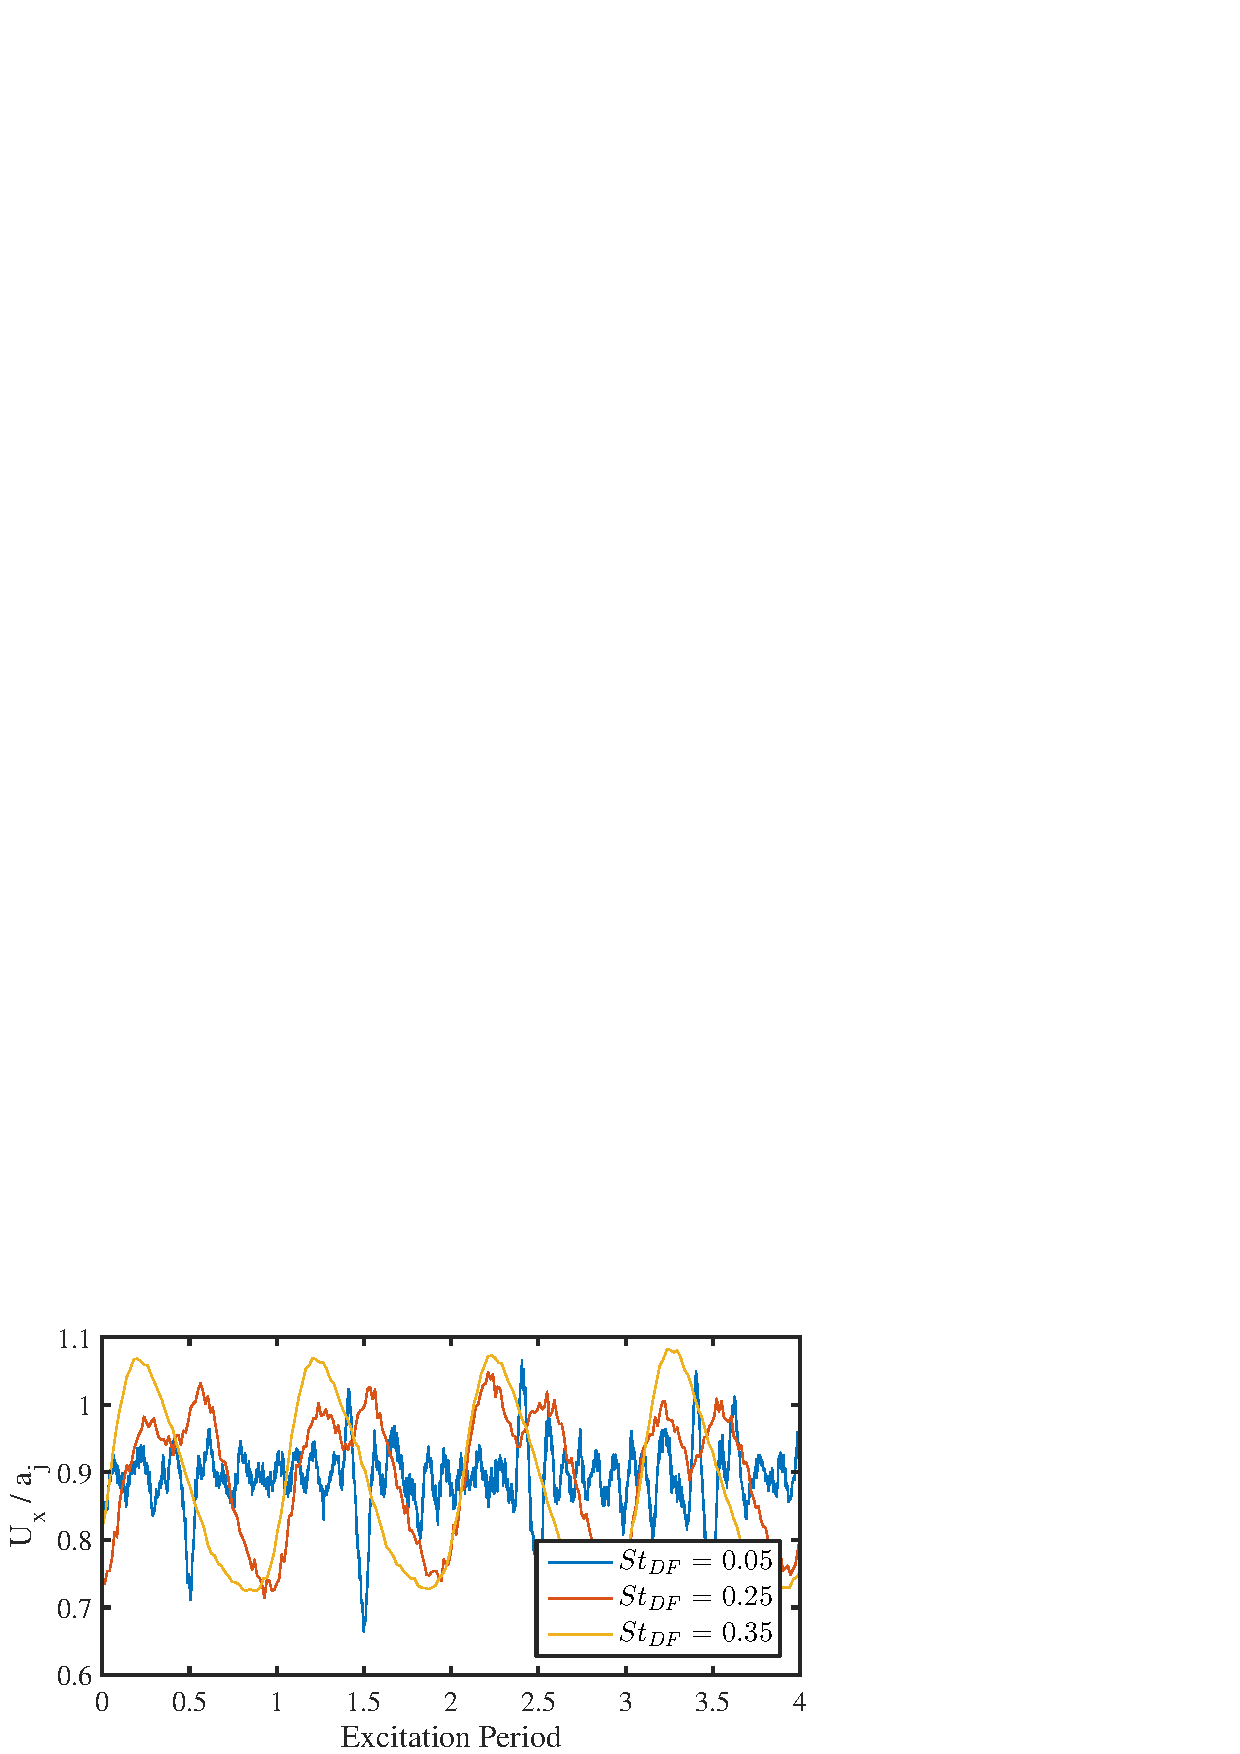
\includegraphics[width=3.5in]{Figures/ch4_centerline_mach_temporal.png} \\
	%		\caption{}
	%		\label{fig:ch4_centerlinemach_temporal}
	%	\end{subfigure}\\
	%	\begin{subfigure}{1\textwidth}
	%		\centering
	\includegraphics[width=3.5in]{Figures/ch4_rawUx_acceleration.png}
	%		\caption{}
	\label{fig:ch4_St005_rawUx_snapshot}
	%	\end{subfigure}
	\caption{Fluctuations associated with the passage of large-scale structures in the axial velocity along the jet centerline at $x/D = 4$ (a) and an arbitrary raw PIV snapshot displaying similar behavior for the $St_{DF}  = 0.05$ jet(b).}
\end{figure}

\subsection{Coherent Structure Merging}
In the simulated subsonic shear layer of \citet{Wei2006}, optimized control for noise mitigation using generalized actuation was implemented using the adjoint perturbation method.
The methodology was able to affect a significant reduction in the emitted noise, though the exact mechanism by which this was accomplished was not immediately clear, even in this highly simplified flow (two-dimensional shear layer).
In \citet{Cavalieri2010b} the same numerical database was investigated with a specific focus on identifying intermittent events related to the noise generation process.
There it was found that the control achieved the majority of the sound reduction by suppressing a single triple vortex interaction, thereby regularizing the flow and preventing the generation of high-amplitude peaks in the acoustic field.
The results of \citet{Kibens1980} also identified vortex merging as a prominent noise source in a (low) subsonic jet.
With this in mind, the evolution of the vortices in the periodically excited jets was analyzed.

\fig{fig:ch4_period_structure_disintegration} illustrates a complete excitation period for the $St_{DF} = 0.25$ excited jet; as before the velocity fields were smoothed prior to computation of the swirling strength, and the results have been phase-averaged over roughly 150 phases.
Previous analysis of the near-field had used two-point correlations between subsequent microphones in order to estimate the convective velocity of the large-scale structures; based on the time-lag for the maximum correlation value, the convective velocity was estimated as $U_c \simeq 0.7 U_j$.
However, the analysis of \citet{Speth2015} in a simulated Mach 0.9 unheated jet found that this method over-predicted the convective velocity; for example, near the end of the potential core two-point correlations in the irrotational near-field produced an estimate of $U_c \simeq 0.67 U_j$ whereas correlations in the \textit{flow}-field produced an estimate of $U_c \simeq 0.64 U_j$.
Essentially, the energy of the acoustic field in the irrotational near-field though small, is non-trivial, and as a result the much higher propagation velocity for the acoustic energy skews the convective velocity estimate to slightly higher values.
By using only the hydrodynamic component of the near-field (produced by the wavelet decomposition of \citet{Crawley2016}), the convective velocity was estimated as $U_c \simeq 0.54 U_j$ near the nozzle exit and $U_c \simeq 0.65 U_j$ near the end of the potential core.
Based on these values, the vortex spacing is expected to be $\simeq 2.6D$ near the end of the potential core.
\begin{figure}
	\centering
	\includegraphics[width=4in]{Figures/ch4_St025_lambda.png}
	\caption{Evolution of the periodic vortex ring ($St_{DF}=0.25$), as visualized using swirling strength. One complete actuation period is shown.}
	\label{fig:ch4_period_structure_disintegration}
\end{figure}

As expected, the excitation produces a periodic roll-up of large-scale structures which, in the downstream region near the end of the potential core, roughly match with the vortex spacing for this frequency (see frame 1 in \fig{fig:ch4_period_structure_disintegration}).
However, in the upstream region ($x/D < 2$) the vortex spacing halves - the LAFPA excitation is in fact producing structures with a frequency associated with the most unstable shear layer frequency, which is significantly higher than the jet column mode frequency.
While this is the first time that this behavior has been observed at the GDTL, it is not terribly surprising if the specifics of LAFPA actuation are considered with respect to the well-known shear layer instability characteristics.
Unlike many other actuators used previously for flow control, the perturbation generated by the LAFPAs is non-sinusoidal and comprised of many higher harmonics than just the fundamental excitation frequency.
These higher harmonics couple to the flow and excite the shear layer instability, which is most unstable at frequencies much higher than the excitation frequencies used in this work.
Therefore, the structures initially formed by the excitation are going to be associated with harmonics of the excitation frequency.
Hence, it is only after merging (or successive mergings) that the passage frequency of the large-scale structures is going to match the fundamental excitation frequency.

In frame 2, the two structures at $x/D = 1$ are beginning to merge.
The trailing structure is inducted inside the preceding structure, and by $x/D \simeq 3$ the merging process is complete.
As the resultant structure convects downstream, the beginning of the breakdown of the vortex is witnessed near $x/D \simeq 4$, similar to the results of the impulsively excited vortex ring and an acceleration of the centerline velocity to slightly supersonic speeds is also observed (\fig{fig:ch4_centerlinemach_temporal}).
Here however, a secondary interaction between structures appears to be occurring, most visibly in frames 5--7. 
Depending on how exactly the coherent vortices are visualized, it appears that a second merging process is commencing here, however the vortices disintegrate before the trailing vortices can be inducted into the first. 
As the vortex at $x/D \simeq 4.5$ is breaking down, the trailing vortex breaks down as well, in fact much more abruptly than the leading vortex; the appearance of structures now matches the excitation frequency.
As the cycle is repeated (beginning again at frame 1), these two vortices (or more accurately, the less coherent, higher-order remnants of them) are no longer individually distinguishable.

Recall that the far-field response of the jet to periodic excitation at $St_{DF}=0.35$ could not be reproduced accurately using a linear superposition of the impulse response.
The vortex dynamics that this excitation frequency produces may thus serve as an insightful contrast for understanding the noise generation phenomena.
A complete excitation cycle for $St_{DF}=0.35$ has been visualized in \fig{fig:ch4_St035_structure_disintegration}.
In this case, two merging processes are now clearly evident.
The first begins just downstream of the nozzle exit, and completes by $x/D \simeq 1.5$; the second begins at $x/D \simeq 2$ and completes relatively quickly, at $x/D \simeq 3$.
It is after this second merging process that the structure spacing now matches the expected wavelength for this excitation frequency ($\lambda \simeq 1.75D$).
As with the lower frequency excitation cases just examined, the dominant vortex (which matches the excitation frequency) undergoes a disintegration beginning around $x/D \simeq 4$.
What is particularly noteworthy here though, is that the disintegration is more rapid for the $St_{DF}=0.05$ and $0.25$ cases than the $St_{DF}=0.35$ case.
In this case, the coherent structure, though severely weakened, is distinguishable over the background noise even downstream of $x/D = 6$.
As with the other excitation frequencies, the core fluid accelerates to supersonic velocities as the large-scale structures pass through the end of the potential core.
\begin{figure}
	\centering
	\includegraphics[width=4in]{Figures/ch4_St035_lambda_evolution.png}
	\caption{Evolution of the periodic vortex ring ($St_{DF}=0.35$), as visualized using swirling strength. One complete actuation period is shown.}
	\label{fig:ch4_St035_structure_disintegration}
\end{figure}

Clearly (and unsurprisingly), the vortex interactions in the periodically-excited jets are far more complex than the impulsively excited jet.
However, as was seen both in terms of the far-field response (\fig{fig:ch3_farfield}) as well as the acoustic source region estimated from the decomposed near-field (\fig{fig:ch3_xcorrOA}), the acoustic fields for $St_{DF}=0.05$ and $St_{DF}=0.25$ show remarkable similarity, at least at angles close to the jet axis.
Therefore, this implies that for this excitation range, the added complexity of the periodic excitation (harmonic structures, vortex merging) are not the primary drivers for noise emission (though they may still play a role).
The consistent, rapid breakdown of the LAFPA-induced structures near $x/D \simeq 4$ and accompanying fluid acceleration in both excited jets appears to be the dominant noise source. 
In contrast, the far-field acoustic response to excitation at $St_{DF}=0.35$ is not accurately reproduced by a linear superposition of the impulse response of the jet.
Analysis of the vortex dynamics demonstrates multiple merging processes occurring for this excitation frequency, and though the dominant vortex breaks down at $x/D \simeq 4$, this process is far less dramatic than in the lower-frequency excitation cases.
In this case, the merging process may in fact be a significant factor in the noise generation process.
In order to more conclusively link this behavior to the noise emission directly, in \sect{sect:source} the aeroacoustic source term will be calculated from the estimated time-resolved velocity fields using a simplified form of Lighthill's acoustic analogy.
\include{sect_acoustic_source}
\section{Conclusions}
The aeroacoustic mechanisms in high-speed, turbulent jets were investigated using simultaneous pressure and velocity measurements of large-scale structures generated by plasma excitation of jet shear layer instabilities.
As the focus of this work was on mixing noise generated by turbulent shear layer structures common to all flow regimes, rather than acoustic emission generated by supersonic flow phenomena, an unheated, Mach 0.9 jet was used.
In the current work, only structures of azimuthal mode zero (axisymmetric ring vortices) were investigated. Previous researchers have identified the axisymmetric mode as the dominant acoustic emission pattern, and this also served to greatly simplify the data acquisition and analysis by eliminating the need to obtain azimuthal velocity components and gradients.

Previous work had identified an impulse response of the jet produced by very low frequency excitation ($St_{DF} \leq 0.05$), a periodic response of the jet produced by higher frequency excitation, and the linear relationship that existed between the two, both in the near-field pressure and the acoustic far-field.
New analysis of the near-field pressure used a wavelet--conditioning technique to extract the coherent signatures for the excited and natural jets.
Results showed clear similarities between the evolution of the signatures of the impulsively-excited structures and that of the natural jet.
The irrotational near-field pressure was then linearly decomposed into its constitutive hydrodynamic and acoustic components via a two-dimensional, spatio-temporal wavelet transform.
Once decomposed, linear correlations between the far-field acoustic signal at $30^\circ$ and the acoustic component of the near-field were computed in order to identify the dominant acoustic source region in the jet based on the measured time-lag for the peak correlation.
In all cases, natural and excited jets, the dominant acoustic source region was found to comprise the upstream region of the jet and end at $x/D \simeq 4$, just upstream of the end of the potential core.
This analysis is meant to identify only the dominant noise source region, and does not mean that no noise is generated outside of this region.
This result is in general accordance with previous results acquired at the GDTL by \citet{Hileman2005}, which identified the acoustic source region using delay-and-sum beamforming with a circular microphone array in the acoustic near-field (that is, far enough such that hydrodynamic pressure effects are negligible, but not in the true geometric far-field of the jet).
In that work, the dominant acoustic source region for an unheated, Mach 1.3 jet was found to be located just downstream of the end of the potential core, and was related to the breakup of large-scale coherent structures as they passed through this region.

The evolution, interactions, and, disintegration of the large-scale structures induced by the plasma excitation were then studied by stochastically-estimating the time-resolved velocity fields from ensemble acquisition of temporally-correlated velocity snapshots and near-field pressure traces.
The velocity snapshots were first decomposed into POD modes and a mapping from the near-field pressure to the POD expansion coefficients was generated by a standard feedforward, backpropagating neural network.
From this, the time-resolved expansion coefficients could be estimated and thus a reduced-order, time-resolved estimate of the velocity field produced.
Results showed that at very low excitation frequencies (impulsive excitation) each plasma pulse generates a single dominant structure, which initially grows rapidly as it convects downstream. 
As the structure nears the end of the potential core, $x/D \simeq 4$, a rapid disintegration of the vortex is observed, coincident with a strong axial acceleration.
As the excitation frequency is increased, a much more complex structure evolution takes form.
At moderate excitation frequencies (periodic forcing), multiple structures are initially formed by the plasma pulse; this is due to the higher-harmonics of the excitation pulse coupling with the most unstable shear layer frequency.
These initial, high-frequency structures quickly undergo a merging process (or multiple mergings) which ultimately produces large-scale coherent structures which are periodic and match the fundamental excitation frequency.
These large-scale structures later undergo a rapid disintegration and acceleration, similar to the impulsive excitation structures, as they convect downstream near the end of the potential core. 

Finally, the aeroacoustic sources were estimated from the time-resolved velocity fields using Ribner's simplified form of Lighthill's acoustic analogy.
This required numerous simplifications to the governing equations, which ultimately degraded the accuracy of the computed aeroacoustic source field.
Unfortunately, this limited interpretation of the results, as the computed far-field acoustic signal did not match well with the measured signal.
The algorithm did reproduce fluctuating acoustic fields of similar amplitude to what was measured experimentally, but the shape of the waveforms only matched in a rough sense.
Fortunately though, broad characteristic changes in the aeroacoustic source fields with excitation could still be identified.
The source fields indicated that the coherent structures produced a convected wavepacket-like event, centered on the jet lipline though reaching into the potential core.
For the individual vortex rings, a clear modulation of the spatial extent and amplitude was observed just upstream of the end of the potential core.
This corresponds to the location at which the coherent ring vortex underwent a rapid disintegration as well as acceleration, and corresponds to the location at which the dominant noise events are emitted per the two-point correlations between the acoustic component of the near-field pressure and the far-field at low polar angles.
For the periodically-excited jet, an additional noise source region is observed, corresponding to the location at which the multiple smaller-scale structures undergo a consistent merging thanks to the highly consistent vortex generation by the excitation.
This secondary source became more prominent as the excitation frequency increased to near the jet column mode frequency and the coherent vortices underwent two merging processes before decaying near the end of the potential core.

The linearity of the acoustic response of the jet (observed in the far-field) to impulsive and low-frequency periodic excitation ($St_{DF} \leq 0.25$), coupled with the observations of the vortex dynamics and acoustic source fields, indicates that the dominant source mechanism for these structures is the rapid modulation of the waveform brought on by the disintegration and acceleration of the large-scale structure as it begins to self-interact near the end of the potential core.
For the unexcited jet, in which ring vortices are highly unstable in the initial shear layer but the large-scale structures have a broad range of frequencies and phase relations to each other (and hence have less chance to merge repeatably), this is likely the dominant noise source mechanism. 
As the excitation frequency increased (to $St_{DF} \simeq 0.35$, which is near the jet column mode frequency), the secondary source mechanism associated with the vortex pairing becomes non-negligible, which results in a modification of the far-field response as it is now a combination of these two source mechanisms.
However, given the broadband nature of the jet turbulence (in terms of both temporal and azimuthal structure), it is unlikely that the vortex merging noise source mechanism is commonly encountered in the highly turbulent jet on a regular basis.
Ultimately, this work indicates that noise suppression may be achieved by seeding the growth of higher-order azimuthal modes, thereby limiting the growth of large-scale coherent structures, which will not undergo a rapid disintegration at the end of the potential core.  

%Acknowledgements should be included at the end of the paper, before the References section or any appendicies, and should be a separate paragraph without a heading. Several anonymous individuals are thanked for contributions to these instructions.

\bibliographystyle{jfm}
\bibliography{master.bib}

\end{document}
